\section{Problem Statement}

\subsection{Event sequences}

\begin{definition}
A \emph{sequence event}, or \emph{event} for short, is defined as a pair $ (A, t) $ where $ A \in \Sigma $ is an event type from a given set of event types $ \Sigma $, and $ t $ is a timestamp integer.
\end{definition}

\begin{definition}
An \emph{event sequence} $ \boldsymbol{s} $ is a triple $ (s, T_s, T_e) $, where $ s $ is an ordered sequence of events
\begin{align*}
s = \langle (A_1, t_1), (A_2, t_2), \, \ldots, \, (A_n, t_n) \rangle
\end{align*}
such that $ t_i \leq t_{i + 1} $ for all $ i = 1, \, \ldots, \, n - 1 $, and any given pair $ (A, t) $ appears at most once.

With $ \boldsymbol{s}_i $ we refer to the pair $ (A_i, t_i) $ in $ s $.

$ T_s $ and $ T_e $ are timestamps such that $ T_s \leq t_1 $ and $ t_n < T_e $. They mark the beginning and the end of the sequence, respectively.

If a sequence event $ (A, t) $ is in $ s $ for a given sequence $ \boldsymbol{s} $, we say that the event \emph{occurs} in $ \boldsymbol{s} $ at timestamp $ t $.
\end{definition}

Figure~\ref{fig:event-sequence} shows a visualization of a possible event sequence.

\newcommand{\examplesequence}
{
    \draw (-5.5,0) -- (5.5,0);

    \foreach \x in {-5.5,-5,...,5.5}
        \draw (\x,0) -- (\x,3pt);

    \foreach \x/\eventtype in {
      -4.5/c,
      -4/f,
      -3.5/b,
      -3/b,
      -1.5/c,
      -0.5/d,
      -0/a,
      1.5/b,
      2.5/e,
      3/a,
      3.5/e,
      4/c}
        \node [font=\vphantom{$ fbd $}] at (\x,1em) {$ \eventtype $};
}

\newcommand{\examplesequencetimestamps}
{
    \foreach \x [evaluate=\x as \timestamp using int((\x*2)+41)] in {-5.5,-3,...,5.5}
    \node at (\x,-1em) {$ \timestamp $};
}

\begin{figure}[h]
\centering

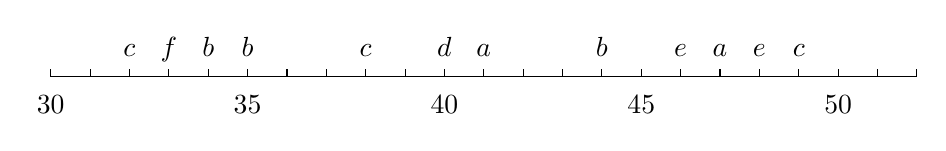
\begin{tikzpicture}

\examplesequence
\examplesequencetimestamps

\end{tikzpicture}

\caption{A visual example of a sequence.}
\label{fig:event-sequence}
\end{figure}

Note that multiple events can occur at the same timestamp, if they have different event types. Some implementations do not allow this, however.

For the sake of simplicity, we use the notation $ s_1 \cdots s_n $ to mean the sequence $ (\langle (s_1, 1), \ldots,\allowbreak(s_n, n) \rangle, 1, n + 1) $.

Since sequences are allowed to be very long, and we are mostly looking for events occurring relatively close to each other, we would like to be able to consider parts of a sequence while ignoring the rest of it. Therefore we use the concept of a window on a sequence.

\begin{definition}
Given a sequence $ \boldsymbol{s} = (s, T_s, T_e) $ and two timestamps $ t_s $ and $ t_e $,
% such that $ t_s < T_e $ and $ T_s < t_e $
we define a \emph{window} on $ \boldsymbol{s} $ to be an event sequence $ \boldsymbol{s}[t_s, t_e) = (w, t_s, t_e) $ where $ w $ contains all events $ (A, t) $ in $ s $ where $ t_s \leq t < t_e $. We call $ \rho = t_s - t_e $ the \emph{width} of the window. Two windows $ \boldsymbol{s}[a, b) $ and $ \boldsymbol{s}[c, d) $ \emph{overlap} if $ [a, b) \cup [c, d) \neq \emptyset $.
\end{definition}

Note that in the previous definition, $ t_s $ and $ t_e $ do not have to be within the sequence. This will be important for some of the algorithms.

Figure~\ref{fig:windows} illustrates a window on the sequence of figure~\ref{fig:event-sequence}.

\begin{figure}[h]
\centering

\begin{tikzpicture}

\examplesequence
\examplesequencetimestamps

\draw [very thick] (1.5,-0.6) -- ++(0,-3pt) -- ++(2.4,0) -- ++(0,3pt);

\draw [->,very thick] (2.75,-0.8) -- ++(0,-0.5);

\draw (1.5,-2) -- ++(2.4,0);

\foreach \x in {1.5,2,...,3.5}
    \draw (\x,-2) -- ++(0,3pt);

\foreach \x/\label in {
    1.5/b,
    2.5/e,
    3/a,
    3.5/e}
    \path (\x,-2) ++(0,1em) node [enoughdamnvspace] {$ \label $};

\path (1.5,-2) ++(0,-1em) node {$ 44 $};

\node [anchor=east] at (1,-2) {Contents of window $ \boldsymbol{s}[44,49) $:};

\end{tikzpicture}

\caption{A window of width 5 on a sequence $ \boldsymbol{s} $.}
\label{fig:windows}
\end{figure}

\subsection{Episodes}

Now we formally define patterns.

\begin{definition}
An \emph{episode} $ \alpha $ is a directed acyclic graph with labelled nodes, that is, $ \alpha = (V, E, lab) $, where $ V = (v_1, \ldots, v_k) $ is the set of nodes, $ E $ is the set of directed edges, and \emph{lab} is a function $ lab \colon V \rightarrow \Sigma $, mapping each node $ v_i $ to an event type. If $ lab(v) = A $, then we say that node $ v $ is of (event) type $ A $, and that $ \alpha $ contains $ A $, or $ A $ is in $ \alpha $.
\end{definition}

We write $ | \alpha | $ to mean the number of nodes in an episode's graph. We call $ | \alpha | $ the \emph{size} of $ \alpha $.

\begin{definition}
A node $ n $ in an episode graph is a \emph{descendant} of a node $ m $ if there is a path from $ m $ to $ n $. Conversely $ m $ is an \emph{ancestor} of $ n $ in that case.
\end{definition}

\begin{definition}
Given a sequence $ \boldsymbol{s} $ and an episode $ \alpha $ we say that $ s $ \emph{covers} $ \alpha $, or $ \alpha $ \emph{occurs in} $ \boldsymbol{s} $, if there is an injective map $ f $ mapping each node $ v_i $ to a valid index such that:
\begin{enumerate}
\item the node $ v_i $ in $ \alpha $ and the corresponding sequence element $ \boldsymbol{s}_{f(v_i)} $ are of the same event type: $ \boldsymbol{s}_{f(v_i)} = lab(v_i) $, and
\item if there is an edge $ (v_i, v_j) $ in $ \alpha $, then we must have $ f(v_i) < f(v_j) $. In other words, the parents of $ v_j $ must occur in $ \boldsymbol{s} $ before $ v_j $. If the mapping $ f $ is surjective, that is, all events in $ \boldsymbol{s} $ are used, we will say that $ \boldsymbol{s} $ is an \emph{instance} of $ \alpha $.
\end{enumerate}
\end{definition}

\begin{definition}
Episodes $ \alpha $ and $ \beta $ are said to be \emph{equivalent} if each sequence that covers $ \alpha $ also covers $ \beta $, and vice versa.
\end{definition}

In this thesis, we'll be limiting ourselves to two subcategories of episodes:
\begin{itemize}
\item \textbf{Parallel episodes.} A parallel episode is an episode for which the set of edges is empty. As such, no constraints are placed on the order in which event types occur in a sequence. An example is shown in figure~\ref{fig:episode-graphs-parallel}. In text we'll write parallel episodes by their event types using the following notation:
\begin{align*}
    \{ A_1, A_2, \ldots, A_n \}
\end{align*}
by which we mean a parallel episode with $ n $ nodes, and the event types are $ A_1 $ through $ A_n $. Note that though the notation reminds strongly of the notation for a mathematical set, it does not actually represent a set: a parallel episode $ \{ a, a, b, c \} $ is not equivalent to an episode $ \{ a, b, c \} $.

\item \textbf{Serial episodes.} A serial episode is an episode for which the edges cause the nodes to have a total order. That way, in any occurrence of a serial episode in a sequence, the event types appear in the same order. Figure~\ref{fig:episode-graphs-serial} shows an example.

% Sometimes it is useful to describe serial episodes in their strict form, in which there is a direct edge between any two nodes. Figure~\ref{fig:episode-graphs-serial-strict} shows a strict episode which is equivalent to the episode in figure~\ref{fig:episode-graphs-serial}.

While serial episodes have a different graph in this form, their meaning is the same, since they enforce the same order on the occurrence of events in the sequence to satisfy an occurrence of a serial episode.

For serial episodes we will use the notation
\begin{align*}
    A_1 \to A_2 \to \cdots \to A_n
\end{align*}
where $ A_i $ is the event type of the $ i $-th node, and a node of event type $ A_i $ is an ancestor of a node of event type $ A_j $ if $ i < j $.

\end{itemize}

\begin{figure}

\begin{subfigure}[b]{\textwidth}
\centering
\begin{tikzpicture}

\node (n 1) [circly,label={$ c $},enoughdamnvspace] at (-3,-3pt) {$ v_1 $};
\node (n 2) [circly,label={$ a $},enoughdamnvspace] at (-1, 3pt) {$ v_2 $};
\node (n 3) [circly,label={$ b $},enoughdamnvspace] at ( 1,-3pt) {$ v_3 $};
\node (n 4) [circly,label={$ b $},enoughdamnvspace] at ( 3, 3pt) {$ v_4 $};

\end{tikzpicture}
\caption{parallel}
\label{fig:episode-graphs-parallel}
\end{subfigure}

\par\bigskip

\begin{subfigure}[b]{\textwidth}
\centering
\begin{tikzpicture}

\node (n 1) [circly,label={$ b $},enoughdamnvspace] at (-3,0) {$ v_1 $};
\node (n 2) [circly,label={$ a $},enoughdamnvspace] at (-1,0) {$ v_2 $};
\node (n 3) [circly,label={$ c $},enoughdamnvspace] at ( 1,0) {$ v_3 $};
\node (n 4) [circly,label={$ d $},enoughdamnvspace] at ( 3,0) {$ v_4 $};

\draw [->] (n 1) -- (n 2);
\draw [->] (n 2) -- (n 3);
\draw [->] (n 3) -- (n 4);

\end{tikzpicture}
\caption{serial}
\label{fig:episode-graphs-serial}
\end{subfigure}

\par\bigskip

\iffalse
\begin{subfigure}[b]{\textwidth}
\centering
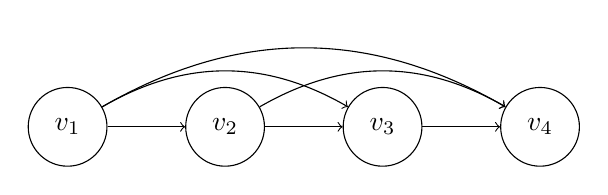
\begin{tikzpicture}

\node (n 1) [circly] at (-3,0) {$ v_1 $};
\node (n 2) [circly] at (-1,0) {$ v_2 $};
\node (n 3) [circly] at ( 1,0) {$ v_3 $};
\node (n 4) [circly] at ( 3,0) {$ v_4 $};

\draw [->] (n 1) -- (n 2);
\draw [->] (n 2) -- (n 3);
\draw [->] (n 3) -- (n 4);

\draw [->] (n 1) to [bend left=30] (n 3);
\draw [->] (n 2) to [bend left=30] (n 4);
\draw [->] (n 1) to [bend left=30] (n 4);

\end{tikzpicture}

\caption{serial, strict}
\label{fig:episode-graphs-serial-strict}
\end{subfigure}
\fi

\caption{An example of an episode graph for each of the episode class we will consider, with the event types shown above the nodes.}

\label{fig:episode-graphs}
\end{figure}

\begin{figure}
\centering

\begin{tikzpicture}

\examplesequence
\examplesequencetimestamps

\foreach \x [evaluate=\x as \timestamp using int((\x*2)+41)] in {-5.5,-5,...,5.5}
    \node (t\timestamp) [inner sep=0] at (\x,1.8em) {};

% serial episode

\node (serC) at (-5,2.5) [smallnode,label={$ c $}] {};
\node (serF) at (-4,2.5) [smallnode,label={$ f $}] {};
\node (serB) at (-3,2.5) [smallnode,label={$ b $}] {};

\draw [->,very thick] (serC) -- (serF);
\draw [->,very thick] (serF) -- (serB);

\draw [->] ([yshift=-3pt]serC.south) .. controls +(0,-1) and +(0,1) .. (t32);
\draw [->] ([yshift=-3pt]serF.south) .. controls +(0,-1) and +(0,1) .. (t33);
\draw [->] ([yshift=-3pt]serB.south) .. controls +(0,-1) and +(0,1) .. (t34);

% parallel episode

\node (parB) at (3,2.6) [smallnode,label={$ b $}] {};
\node (parE1) at (2,1.8) [smallnode,label={$ e $}] {};
\node (parE2) at (4.5,2.4) [smallnode,label={$ e $}] {};
\node (parC) at (3.5,2) [smallnode,label={$ c $}] {};

\draw [->] ([yshift=-3pt]parB.south) .. controls +(0,-1) and +(0,1) .. (t44);
\draw [->] ([yshift=-3pt]parE1.south) .. controls +(0,-0.5) and +(0,0.5) .. (t46);
\draw [->] ([yshift=-3pt]parE2.south) .. controls +(0,-1) and +(0,1) .. (t48);
\draw [->] ([yshift=-3pt]parC.south) .. controls +(0,-0.5) and +(0,0.5) .. (t49);

\end{tikzpicture}

\caption{Showing an occurrence of a serial episode $ c \to f \to b $ and an occurrence of a parallel episode $ \{ b, c, e, e \} $ in the sequence of figure~\ref{fig:event-sequence}.}
\label{fig:occurrences}
\end{figure}

Because we only consider parallel and serial episodes, it is easy to represent an episode in a data structure---we don't need to explicitly store a graph with nodes and edges:
\begin{itemize}
\item Parallel episodes can be stored in an array, where each element is simply the event type of the episode. Strictly speaking, the order of the elements in the array doesn't matter, but it can be useful for them to follow some order on the set of event types. In that way each parallel episode has a unique array representation. Figure~\ref{fig:parallel-representation} shows the representation visually.

\tikzset{circly/.style={draw,circle,minimum size=1cm},
    arraycell/.style={draw,rectangle,minimum size=1cm,node distance=0}}

\begin{figure}[h]
\centering

\begin{tikzpicture}

\node (n 1) [circly,label=above:$ c $] at (-3,-3pt) {$ v_1 $};
\node (n 2) [circly,label=above:$ a $] at (-1, 3pt) {$ v_2 $};
\node (n 3) [circly,label=above:$ b $] at ( 1,-3pt) {$ v_3 $};
\node (n 4) [circly,label=above:$ a $] at ( 3, 3pt) {$ v_4 $};

\node [left=of n 1] {episode graph};

\draw [->] (0,-1) -- node [left=0.5cm] {sort the event types into an array} +(0,-1.5);

\node (a 1) [arraycell,enoughdamnvspace] at (-2,-3.5) {$ a $};
\node (a 2) [arraycell,right=of a 1,enoughdamnvspace] {$ a $};
\node (a 3) [arraycell,right=of a 2,enoughdamnvspace] {$ b $};
\node (a 4) [arraycell,right=of a 3,enoughdamnvspace] {$ c $};

\end{tikzpicture}

\caption{A parallel episode's graph representation, with the label of each node shown above, and its array representation.}

\label{fig:parallel-representation}
\end{figure}

\item Serial episodes can also be stored in an array, but here the order of the elements is defined by the edges of the episode. That is, the event types are ordered according to a topological sort of the nodes. Figure~\ref{fig:serial-representation} shows this visually.
\end{itemize}

\begin{figure}[h]
\centering

\begin{tikzpicture}

\node (n 1) [circly,label=above:$ a $] at (-3,0) {$ v_1 $};
\node (n 2) [circly,label=above:$ c $] at (-1,0) {$ v_2 $}
    edge [pre] (n 1);
\node (n 3) [circly,label=above:$ b $] at (1, 0) {$ v_3 $}
    edge [pre] (n 2);
\node (n 4) [circly,label=above:$ a $] at (3, 0) {$ v_4 $}
    edge [pre] (n 3);

\node [left=of n 1] {episode graph};

\draw [->] (0,-1) -- node [left=0.5cm,align=right] {store event types into array,\\preserving toplogical ordering} +(0,-1.5);

\node (a 1) [arraycell,enoughdamnvspace] at (-2, -3.5) {$ a $};
\node (a 2) [arraycell,right=of a 1,enoughdamnvspace] {$ c $};
\node (a 3) [arraycell,right=of a 2,enoughdamnvspace] {$ b $};
\node (a 4) [arraycell,right=of a 3,enoughdamnvspace] {$ a $};

\end{tikzpicture}

\caption{A serial episode's graph representation, with the label of each node shown above, and its array representation.}
\label{fig:serial-representation}
\end{figure}

When discussing the algorithms we will mostly consider their array representation, and address the $ i $-th element of an episode array $ \alpha $ with $ \alpha [i] $.

\begin{definition}
Given two episodes $ \alpha $ and $ \beta $, we say that $ \alpha $ is a \emph{subepisode} of $ \beta $, denoted $ \alpha \subseteq \beta $, if the set of all sequences that cover $ \beta $ is a subset of the set of all sequences that cover $ \alpha $. $ \alpha $ is a \emph{proper subepisode} of $ \beta $ if $ \alpha \subseteq \beta $ and $ \alpha $ and $ \beta $ are not equivalent. In that case we can write $ \alpha \subset \beta $.
\end{definition}

Of course, considering all event sequences that cover an episode is an impossible task, so the above definition does not give rise to a practical way of determining whether one episode is a subepisode of another. Instead we must look at the episodes themselves, and reason about all of the ways in which they might occur in a sequence. For parallel and serial episodes, it is quite straightforward to do so, as described below. More general cases have been reasoned about~\cite{tatti12}, but are beyond the scope of this thesis.

\begin{itemize}
\item A parallel episode $ \alpha $ is a subepisode of a parallel episode $ \beta $ if:
\begin{enumerate}
\item $ | V(\alpha) | \leq | V(\beta) | $, and
\item for each event type $ A $ in $ \alpha $, the number of nodes $ v $ in $ \alpha $ for which $ lab(v) = A $, is no greater than the number of nodes for which the same holds in $ \beta $.
\end{enumerate}
\item For serial episodes, the above is also a condition. Additionally, for each node $ v $ in $ \alpha $ of type $ A $ that is an ancestor of a node $ u $ of type $ B $, $ \beta $ must also have two nodes for which the node with event type $ A $ precedes the node with event type $ B $. Put more simply, the ordering of event types must be preserved.
\end{itemize}

\begin{definition}
Given two episodes $ \alpha $ and $ \beta $ such that $ \beta \subset \alpha $, we can express an \emph{association rule} $ \alpha \Rightarrow \beta $. We call $ \alpha $ the \emph{head} of the rule, and $ \beta $ the \emph{tail} of the rule.
\end{definition}

Given an association rule $ \alpha \Rightarrow \beta $, we can define a confidence value $ c(\alpha \Rightarrow \beta) $, which expresses the likelihood of finding an occurrence of $ \beta $, given that we have an occurrence of $ \alpha $ in a sequence. So, intuitively, the confidence value of an association rule gives an indication of how well an occurrence of the head of the rule ``predicts'' an occurrence of the tail.

\subsection{Interestingness measures}

Having discussed episodes occurring in event sequences, we would now like to be able to express how interesting an episode is in regard to a sequence.

Traditionally, the most common interpretation of \emph{interestingness} is frequency, which expresses how often an episode occurs in the sequence. The more often an episode occurs, the more interesting it is considered to be.

Exactly how the frequency of an episode in a sequence should be defined, is not immediately clear in sequential pattern mining. We will present three methods to measure the frequency of an episode and the confidence of an association rule. In a later section, we implement a mining algorithm based on them.

We'll also briefly discuss some interestingness measures that are not based on frequency.

\subsubsection{Fixed windows}

The first frequency measure we discuss was first proposed in~\cite{winepi97}, and is based on windows of a fixed length.

\begin{definition}
Given a window size $ \rho $ and a sequence $ \boldsymbol{s} $, we define the \emph{fixed-window frequency} of an episode $ \alpha $ in $ \boldsymbol{s} $, denoted $ fr_f(\alpha, \boldsymbol{s}) $, to be the number of windows of size $ \rho $ in $ \boldsymbol{s} $ covering the episode:
\begin{align*}
fr_f(\alpha, \boldsymbol{s}) = | \{ \boldsymbol{s}[i, i + \rho) \mid \boldsymbol{s}[i, i + \rho) \text{ covers } \alpha \} |
\end{align*}
\end{definition}

At first sight, counting the number of windows which cover the episode might seem a good approach---intuitively, if an episode occurs in many windows, then it must be frequent. However, upon closer inspection, the frequency values it produces are often counterintuitive, as they don't reflect very well how many occurrences there really are.

Figure~\ref{fig:fwi-example} shows all of the windows of size 8 that cover the episodes shown in figure~\ref{fig:occurrences}. We observe that $ fr_f(\{ a, a, b, c \}) = 6 $, and $ fr_f(c \to f \to b) = 3 $. We can immediately see a drawback to this definition of frequency: the frequency values are highly dependent on the window size. If we were to choose a window size of $ 6 $ instead, then $ fr_f(\{ a, a, b, c \}) = 6 $ and $ fr_f(c \to f \to b) = 1 $. We also see that the more an occurrence is spread out, the fewer windows cover it, and consequently the lower the frequency will be.

\begin{figure}
\centering

\begin{tikzpicture}

\examplesequence

\foreach \x [evaluate=\x as \timestamp using int((\x*2)+41)] in {-5.5,-5,...,5.5}
    \node (t\timestamp) [inner sep=0] at (\x,1.8em) {};

%% draw occurrence proofs again
% serial episode

\node (serC) at (-5,2.5) [smallnode,label={$ c $}] {};
\node (serF) at (-4,2.5) [smallnode,label={$ f $}] {};
\node (serB) at (-3,2.5) [smallnode,label={$ b $}] {};

\draw [->,very thick] (serC) -- (serF);
\draw [->,very thick] (serF) -- (serB);

\draw [->] ([yshift=-3pt]serC.south) .. controls +(0,-1) and +(0,1) .. (t32);
\draw [->] ([yshift=-3pt]serF.south) .. controls +(0,-1) and +(0,1) .. (t33);
\draw [->] ([yshift=-3pt]serB.south) .. controls +(0,-1) and +(0,1) .. (t34);

% parallel episode

\node (parB) at (3,2.6) [smallnode,label={$ b $}] {};
\node (parE1) at (2,1.8) [smallnode,label={$ e $}] {};
\node (parE2) at (4.5,2.4) [smallnode,label={$ e $}] {};
\node (parC) at (3.5,2) [smallnode,label={$ c $}] {};

\draw [->] ([yshift=-3pt]parB.south) .. controls +(0,-1) and +(0,1) .. (t44);
\draw [->] ([yshift=-3pt]parE1.south) .. controls +(0,-0.5) and +(0,0.5) .. (t46);
\draw [->] ([yshift=-3pt]parE2.south) .. controls +(0,-1) and +(0,1) .. (t48);
\draw [->] ([yshift=-3pt]parC.south) .. controls +(0,-0.5) and +(0,0.5) .. (t49);

% windows

\newcommand{\windowthingy}[1]
{
    \draw #1 -- ++(0,-3pt) -- ++(3.9,0) -- ++(0,3pt);
}

\windowthingy{(-7,-5pt)}
\windowthingy{(-6.5,-10pt)}
\windowthingy{(-6,-15pt)}
\windowthingy{(-5.5,-20pt)}
\windowthingy{(-5,-25pt)}
\windowthingy{(-4.5,-30pt)}

\windowthingy{(0.5,-5pt)}
\windowthingy{(1,-10pt)}
\windowthingy{(1.5,-15pt)}

\end{tikzpicture}

\caption{All of the windows of size 8 that cover two episodes in a sequence; a parallel episode $ \{a, a, b, c \} $ and a serial episode $ c \to f \to b $.}
\label{fig:fwi-example}
\end{figure}

\begin{definition}
Given a window size $ \rho $ and episodes $ \alpha $ and $ \beta $, such that $ \alpha \subset \beta $, we define the \emph{fixed-window confidence} of the association rule $ \alpha \Rightarrow \beta $, denoted $ c_f(\alpha \Rightarrow \beta) $, to be the ratio of their respective frequencies:
\begin{align*}
c_f(\alpha \Rightarrow \beta) = \frac{ fr_f(\beta) }{ fr_f(\alpha) }
\end{align*}
\end{definition}

Given that the fixed-window frequency gave unintuitive results for episodes, and that the fixed-window confidence is based on the fixed-window frequency, it should be no surprise that the confidence values for the fixed-window confidence can also be unintuitive.

Consider again the occurrence of the parallel episode in figure~\ref{fig:fwi-assoc-example}. With $ \rho = 8 $ as in the figure, $ fr_f(\{ e, e \}) = 6 $.

\begin{figure}
\centering

\begin{tikzpicture}

\clip (0,-10) rectangle (10,10);

\examplesequence

\foreach \x [evaluate=\x as \timestamp using int((\x*2)+41)] in {-5.5,-5,...,5.5}
    \node (t\timestamp) [inner sep=0] at (\x,1.8em) {};

%% draw occurrence proofs again
% serial episode

\node (serC) at (-5,2.5) [smallnode,label={$ c $}] {};
\node (serF) at (-4,2.5) [smallnode,label={$ f $}] {};
\node (serB) at (-3,2.5) [smallnode,label={$ b $}] {};

\draw [->,very thick] (serC) -- (serF);
\draw [->,very thick] (serF) -- (serB);

\draw [->] ([yshift=-3pt]serC.south) .. controls +(0,-1) and +(0,1) .. (t32);
\draw [->] ([yshift=-3pt]serF.south) .. controls +(0,-1) and +(0,1) .. (t33);
\draw [->] ([yshift=-3pt]serB.south) .. controls +(0,-1) and +(0,1) .. (t34);

% parallel episode

\node (parB) at (3,2.6) [smallnode,label={$ b $}] {};
\node (parE1) at (2,1.8) [smallnode,label={$ e $}] {};
\node (parE2) at (4.5,2.4) [smallnode,label={$ e $}] {};
\node (parC) at (3.5,2) [smallnode,label={$ c $}] {};

\draw [->] ([yshift=-3pt]parB.south) .. controls +(0,-1) and +(0,1) .. (t44);
\draw [->] ([yshift=-3pt]parE1.south) .. controls +(0,-0.5) and +(0,0.5) .. (t46);
\draw [->] ([yshift=-3pt]parE2.south) .. controls +(0,-1) and +(0,1) .. (t48);
\draw [->] ([yshift=-3pt]parC.south) .. controls +(0,-0.5) and +(0,0.5) .. (t49);

% windows

\newcommand{\windowthingy}[1]
{
    \draw #1 -- ++(0,-3pt) -- ++(3.9,0) -- ++(0,3pt);
}

\windowthingy{(-7,-5pt)}
\windowthingy{(-6.5,-10pt)}
\windowthingy{(-6,-15pt)}
\windowthingy{(-5.5,-20pt)}
\windowthingy{(-5,-25pt)}
\windowthingy{(-4.5,-30pt)}

\windowthingy{(0.5,-5pt)}
\windowthingy{(1,-10pt)}
\windowthingy{(1.5,-15pt)}

\end{tikzpicture}

\label{fig:fwi-assoc-example}
\end{figure}

\subsubsection{Minimal windows}

\begin{definition}
Given a sequence $ s $ and an episode $ G $, a window $ s[a, b] $, is called a \emph{minimal window} of $ G $ in $ s $, if:
\begin{itemize}
\item $ len(s[a, b]) \leq \rho $, $ s[a, b] $, and
\item no proper subwindow of of $ s[a, b] $ covers $ G $.
\end{itemize}
We define beginning, end ... % TODO figure out definitions (inclusive-exclusive end-timestamp)

We denote the set of all minimal windows of $ G $ in $ s $ with $ mw(G; s) $, or simply $ mw(G) $ if $ s $ is known from the context. Given a set of minimal windows $ W $, we define a function $ dis(W) $ to be equal to 1 if all windows in $ W $ are pairwise disjoint, and 0 otherwise.
\end{definition}

\begin{definition}
The \emph{disjoint-window frequency} of an episode $ G $ in a sequence $ s $, denoted $ fr_m(G) $, is defined as the maximal number of non-overlapping minimal windows within $ s $ that contain episode $ G $. Formally:
\begin{align*}
fr_m(G) = \text{max} \{ | W | \mid W \subseteq mw(G) \wedge dis(W) = 1 \}
\end{align*}
\end{definition}

\begin{definition}
Given episodes $ X $ and $ Y $, such that $ X \subset Y $, and a minimal window $ s[a, b] $ of episode $ X $. Assume there exists a minimal window $ s[c, d] $ of $ Y $ such that $ c \leq a $ and $ b \leq d $, then we define the \emph{minimal-extensibility} of occurrence $ s[a, b] $ of $ X $ into an occurrence of $ Y $ as
\begin{align*}
ext_m(s[a, b], X, Y) = 1
\end{align*}
If there exists no such minimal window of $ Y $, we define $ ext_m(s[a, b], X, Y) = 0 $.
\end{definition}

\subsubsection{Weighted minimal windows}

\begin{definition}
The \emph{total weight} of a set of windows $ W $ in a sequence $ s $, denoted $ tw(W) $, is defined as
\begin{align*}
tw(W) = \sum_{w \in W}{\frac{1}{len(w)}}
\end{align*}
The \emph{weighted-window frequency} of an episode $ G $ in a sequence $ s $, denoted $ fr_w(G) $, is defined as
\begin{align*}
fr_w(G) = \text{max} \{ tw(W) | W \subseteq mw(G), dis(W) = 1 \}
\end{align*}
\end{definition}

\subsubsection{Other interestingness measures}
